\newgeometry{left=4.5cm, right=4.5cm,bottom=4cm, top=4cm}

\chapter{Higgs Bosons in Standard Model and MSSM} \label{chap:theory}

 \vspace{2cm}

In this chapter,   the theoretical concepts relevant for the experimental search presented in this thesis are introduced.
A brief overview of the Standard Model of particle physics is given in Section~\ref{sec:SM} based on reference~\cite{Altarelli}. 
Among  the extensions of the Standard Model, the minimal supersymmetric 
extension (MSSM) is  theoretically favoured  as one of the most predictive scenarios.
The MSSM is introduced in Section~\ref{sec:MSSM} with  emphasis on the Higgs boson sector
 based on  references~\cite{SusyPrimer,Djuadi}.
Finally, a review of the phenomenological aspects of the MSSM Higgs boson production and decays is given 
in Section~\ref{sec:pheno} based on reference~\cite{LHCxsec}.
%In section... introduction is given based on~\cite{Altarelli}, 
%This chapter is devoted to introduce the the Minimal Supersymmetric 
%extension of the Standard Model (MSSM) whit focus on  its Higgs sector.
%In section... introduction is given based on~\cite{Altarelli}, 

\restoregeometry

\clearpage

\section{The Standard Model of Particle Physics} \label{sec:SM}
\subsection{Introduction}
A detailed description of the Standard Model (SM) of particle physics can be found in reference~\cite{Peskin}. A brief overview is
given below.

The SM of particle physics desrcibes the interactions of the known fermionc matter particles, quarks and leptons, via the
strong, the electromagnetic and the weak forces based on  the principle of local gauge invariance,  i.e. invariance under  
phase  transformations depending  on the space-time coordinates.
The gravitational force is negligible in atomic and nuclear physics since 
quantum gravity effects are expected only at very high energies at the  Planck scale of $\sim 10^{19}$~GeV.

% is a theory aimed to describe and quantitatively predict
%the phenomenology of fundamental particle interactions. At the quantum  level the spectrum of all interactions between matter and 
%radiation can be understood in terms of three fundamental forces: the strong, the electromagnetic
%and the weak forces. These interactions are described by a local relativistic quantum field theory, where 
%a field with suitable transformation properties under the Lorentz group is associated to each particle.
%5The theory is based on the principle of gauge invariance, i.e. invariance under  symmetry  transformations    
%that operate on basic internal degrees of freedom and depend on the space-time coordinate.
%The gravitational force is negligible in atomic and nuclear physics, since the
%quantum effects of gravity are expected only at very high energies corresponding to the Planck mass $E \sim M_{Planck} c^2 \sim 10^{19}$~GeV.

The gauge  symmetries of the SM are described by the group $SU(3)_c \otimes SU(2)_L \otimes U(1)_Y$ which has $8+3+1=12$
generators and gauge fields. The electromagnetic and weak interactions~\cite{EW1,EW2,EW3}  are described  by the 
$SU(2)_L \otimes U(1)_Y$ symmetry group, while $ SU(3)_c$ is the group of the strong colour forces of Quantum Chromodinamics (QCD)~\cite{qcd1}.
A vector boson is associated to each generator of the gauge symmetry groups of the SM acting as  mediator of the interaction.
Eight gluons are associated to the $ SU(3)_c$ colour group, while  four gauge bosons, $W^{\pm}$,
$Z^0$ and $\gamma$, are associated to the electroweak symmetry $SU(2)_L \otimes U(1)_Y$. 
The gluons and the photon are massless while the remaining weak gauge bosons have mass. 
These masses are introduced without spoiling the electroweak gauge symmetry 
via the mechanism of spontaneous symmetry breaking~\cite{ENGLERT,HIGGS,HIGGS2,HIGGS3,kibble}, an additional complex scalar field is required for this
purpose and give rise to a new scalar particle, the Higgs boson, which interacts with other particles with a stregth proportional to their masses.

Quarks  are subject to all SM interactions. Each quark flavour  is a colour triplet and carries 
electroweak charges including electric charges of $+2/3$ and $-1/3$ for up-type and  down-type quarks respectively.
Leptons are colourless but have electroweak charges. The electrons, muons and $\tau$ leptons carry  electric charge  $-1$,
while the associated neutrinos $\nu_e$, $\nu_{\mu}$ and $\nu_{\tau}$ are electrically neutral. Opposite sign 
electric charges are carried by the respective anti-particles.
Quarks and leptons group in three  ``generations'' with equal charge quantum numbers but increasing masses.

\subsection{The Higgs Mechanism in the SM}
The Higgs mechanism extends the Standard Model by a complex scalar field $\Phi$, in its minimal realisation~\cite{ENGLERT,HIGGS,HIGGS2,HIGGS3,kibble}
one scalar $SU(2)_L$ doublet 
\begin{equation}
\Phi = \begin{pmatrix} \phi^+ \\ \phi^0 \end{pmatrix} 
\end{equation}
with four degrees of freedom and weak hypercharge $Y\, = \,+1$ is introduced. The Higgs potential
\begin{equation}
V(\Phi) = \mu^2\Phi^\dagger\Phi +\lambda(\Phi^\dagger\Phi)^2 \,,
\end{equation} 
with the mass parameter $\mu$ and self coupling $\lambda$ is invariant under $SU(2)_L \otimes U(1)_Y$ symmetry transformations.
For $\mu^2 <0$  the scalar field has an infinite set of degenerate ground states.  If a non vanishing vacuum expectation value is choosen
for the neutral component of the scalar filed $\Phi$, the  $SU(2)_L \otimes U(1)_Y$ symmetry is spontaneusly broken with the electromagnetic gauge symmetry
$U(1)_Q$ remaining as a symmetry of the ground state. Therefore, three of the original four degrees of freedom 
of the scalar field are absorbed as longitudinal polarization states of the $W^{\pm}$ and $Z$ bosons, which in this way acquire their 
masses, while the photon remains massless. The remaining degree of freedom corresponds to a physical massive scalar particle, the Higgs boson.

The masses of the fermions can be generated by means of Yukawa couplings to the Higgs field $\Phi$~\cite{yukawa}.


\subsection{Precision Tests and Limitations of the SM}

The Standard Model has been successfully tested in a vast number of experiments over a wide range of energies during the last decades.
Precision tests of the electroweak theory performed at LEP, SLC and Tevatron accellerators~\cite{smtest}  
confirmed that the couplings of quark and leptons to the weak gauge bosons $W^{\pm}$  and $Z$ fully agree 
with the predictions of the SM. Due to the high experimental accuracy of the per-mille level, not only the tree-level
predictions, but also the impact of quantum corrections have been verified. 
Measurements of weak hadron decays togheter with several other experimental results~\cite{pdg}
provide additional tests of the Standard Model at low energies. 
The recent discovery at the LHC of a Higgs boson   with a mass of about $125$~GeV \cite{AHiggsO,CHiggsO} 
is another success of the SM. The measured mass is in agreement with the allowed range from the combined measurement 
of electroweak observables~\cite{gfitter}. The spin and coupling strenght of the new boson are also 
in good agreement with the SM predictions for the measured mass.

%Among all the parameters of the Standard Model only few of them presents 
Tension between the SM predictions and  experimental data is found for only very few observables. 
The most significant discrepancies, of slightly above three standard deviations, are observed for the anomalous magnetic moment 
of the muon $a_{\mu}$~\cite{gminus2} and for the forward-backward asymmetry in bottom quark production at LEP~\cite{smtest}
and in the top quark production at the Tevatron~\cite{FBasymmetry}.   


Inspite of this success, the Standard Model is conceptually unsatisfactory due to a number of deficiencies and is
widely believed to be an effective theory valid only for energies up to the electroweak scale. In addition to the fact that 
the SM does not  include the  gravitational force, it does not explain the pattern of fermion masses and, in its simplest 
version, does not allow for neutrino masses, the theory has other deficiencies indicating the need 
for new physics beyond the Standard Model (BSM). Some of the most important are discussed below.
%\begin{itemize}
%\item
\paragraph{Hierarchy and Fine-Tuning Problem} The radiative corrections to the Higgs boson mass introduce quadratic divergences in  
	the cut-off energy scale $\Lambda$ up to which the theory is considered to be valid~\cite{Lambda}.
	If the cut-off scale chosen is the Planck scale or the GUT scale (see below), a fine tuning of the 
	higher order corrections is needed with an unnaturally high precision of $\mathcal{O}(10^{-30})$ 
	to give a  Higgs boson mass near the electroweak scale $\mathcal{O}(100\,GeV)$ as measured~\cite{Hierarchy1,Hierarchy2,Hierarchy3}.
%	The SM provides no satisfactory answer to the question on  how these cancellations can occur and why $\Lambda >> M_{EW}$. These problems are
%	referred to as the fine-tuning and hierarchy problem~\cite{Hierarchy1,Hierarchy2,Hierarchy3}.

	%Supersymmetry was first introduced to answer this question, indeed, the new symmetry prevents the Higgs boson mass to acquire very large 
	%radiative corrections, the quadratic divergent loop of the SM particles are exactly cancelled by the loop contribution 
	%of the corresponding partners, solving in this way the hierarchy problem~\cite{Djuadi5}.

%\item
\paragraph{Dark Matter}   The SM does not contain a particle candidate for the observed large contribution 
	of dark non-barionic  matter to the energy density of the Universe~\cite{darkmatter1,darkmatter2,darkmatter3}. 
	Dark matter candidates have to be massive, stable and only weakly interacting particles. 
	%Supersymmetry models,  provided with R-parity conservation,
	%provides a natural candidate for Dark Matter, which would be then the lightest SUSY particle which cannot further decay.

%\item 
\paragraph{Gauge Unification Problem}	Another unsatisfactory aspect of the SM is that the electroweak and strong 
	gauge couplings do not evolve to the same value at high energies. Motivated by the successful unification of electromagnetic and weak
	interaction, the existence of a Grand Unified Theory (GUT) has been 
	suggested~\cite{GUT1,GUT2}, which predicts the unification of  the three gauge symmetries of the SM  in a single gauge group with just one coupling constant
	 at the GUT energy scale of about $10^{16}$~GeV.
	%The particle spectrum in SUSY, instead, contributes to the renormalisation group evolution of the three gauge couplings constants and 
	%favours them to meet at energies around $10^{16}$ GeV~\cite{djuadi4}. 

%\end{itemize}
\vspace{0.5cm}
Among many possible extensions of the SM, supersymmetry is  theoretically  favoured  
as it provides natural solutions to the above problems. 
As discussed in Section~\ref{sec:MSSM}, it can solve  the hierarchy problem, provide a suitable dark matter particle candidate 
and predicts unification of the three SM gauge couplings at the GUT scale.


% the conceptual situation with the
%standard model is unsatisfactory for quite a few deficiencies:
%– the smallness of the electroweak scale v ∼ 246GeV << MPl (the ‘hierarchy problem’);
%– the large number of free parameters (gauge couplings,
%vacuum expectation value, MH, fermion masses,
%CKM matrix elements), which are not predicted but have
%to be taken from experiments;
%– the pattern that occurs in the arrangement of the
%fermion masses;
%– the missing way to connect to gravity.
%
%-Dark matter
%
%-neutrino masses

 
\section{The Minimal Supersymmetric Standard Model}\label{sec:MSSM}
\subsection{Introduction to the MSSM}
Supersymmetry (SUSY)~\cite{Susy1,Susy2,Susy3} was first introduced in the 1970s as a new symmetry relating fermions and bosons.
The SUSY generators $\mathcal{Q}$ transform fermion fields into boson and vice versa:
\begin{equation}
\mathcal{Q}|\text{Fermion}\rangle = |\text{Boson}\rangle, ~ ~ ~ \mathcal{Q}|\text{Boson}\rangle = |\text{Fermion}\rangle\,.
\end{equation}
In a supersymmetric extension of the SM,  each of the known fundamental particle states 
is  either in  a chiral or gauge \emph{supermultiplet} togheter with a superpartner with spin differing by unit 1/2.

SUSY naturally solves the hierarchy problem since the quadratically divergent loop contributions to the Higgs mass from  SM 
particles are cancelled  by  loop contributions from the superpartners. 
The quark and lepton  superpartners are labelled by adding an ``s'' in front of the name, standing for scalar. 
The SM gauge bosons also have spin-1/2 partners named by adding ``ino'' as suffix to the name. 
The symbol of superpartners results from adding ``($\tilde{ ~ }$)'' to the SM symbol.
The SUSY particles share the same couplings with their SM partners. 
Since the left- and right-handed components of fermions shows to transform differently under the weak $SU(2)$ gauge symmetry,
their superpartner inherit this feature.

The  minimal supersymmetric extension of the Standard Model  (MSSM)~\cite{MSSM1,MSSM2,MSSM3,MSSM4,MSSM5,MSSM6}, 
is defined by requiring the minimal gauge group as in the SM and 
minimal particle content: the three generations of fermions (without right-handed neutrinos) and gauge bosons of the SM  and two Higgs doublets 
with their superpartners. The  chiral and gauge supermultiplets of the MSSM 
are listed in Tables~\ref{tab:chiralsup} and~\ref{tab:gaugesup}, respectively.
The superpartners of the Higgs bosons, the \emph{higgsinos},  the \emph{wino} and \emph{bino} 
mix with each other resulting in the following mass eigenstates: two charginos $\chi_{1,2}^\pm$ and four neutralinos $\chi_{1,2,3,4}^0$.

\begin{table}
\caption{The chiral supermultiplets of the first generation in the minimal supersymmetric Standard Model (see ref.~\cite{SusyPrimer}).
	 The spin-0 fields are complex scalars 	and the spin-1/2  left-handed two-component Weyl spinors.} \vspace{3mm}
\begin{center}
\renewcommand{\arraystretch}{1.5}
\begin{tabular}{c|ccc}
\hline%\noalign{\smallskip}
Names 			&Supermultiplets	&	Spin 1/2  		& Spin 0 \\%[0.1cm]
\hline%\noalign{\smallskip}		
quarks, squarks		& $Q$ 			&	$(u_L ~ d_L)$		& $( \tilde{u}_L ~ \tilde{d}_L)$ \\%[0.1cm]
			& $\bar{u}$		& 	$u_R^{\dagger}$ 	& $\tilde{u}_R^*$ \\%[0.1cm]
			& $\bar{d}$		& 	$d_R^{\dagger}$ 	& $\tilde{d}_R^*$ \\%[0.1cm]
\hline%\noalign{\smallskip}
leptons, sleptons	& $L$			&   	$(\nu ~ e_L)$ 		&  $( \tilde{\nu} ~ \tilde{e}_L)$\\%[0.1cm]
			& $\bar{e}$		&	$e_R^{\dagger}$         & $\tilde{e}_R^*$ \\%[0.1cm]
\hline%\noalign{\smallskip}
Higgs bosons, Higgsinos	& $H_1$			&	$( \tilde{H}_1^0 ~ \tilde{H}_1^-)$  &	$( H_1^0 ~ H_1^-)$ \\%[0.1cm]	 
			& $H_1$			&	$( \tilde{H}_2^+ ~ \tilde{H}_2^0)$  &	$( H_2^+ ~ H_2^0)$ \\%[0.1cm]	 
\hline
\end{tabular}
\label{tab:chiralsup}
\end{center}
\end{table}

\begin{table}
\caption{ The gauge supermultiplets in the minimal supersymmetric Standard Model (see ref.~\cite{SusyPrimer}).} \vspace{3mm}
\begin{center}
\renewcommand{\arraystretch}{1.5}
\begin{tabular}{c|ccc}
Names			&Supermultiplets& Spin 1 		&	Spin 1/2 \\
\hline
gluons, gluinos		&$G_a$ (a =1,...,8)	& $g$			& $\tilde{g}$	\\
W bosons, winos		& $W_a$ (a=1,...,3)	& $W^{\pm} \,,\, W^0$	& $\tilde{W}^{\pm} \,,\,\tilde{W}^0$ \\
B boson, bino		&$B$			& $B^0$			& $\tilde{B}^0$ \\
\hline
\end{tabular}
\label{tab:gaugesup}
\end{center}
\end{table}

\subsubsection{$R$-parity conservation}
The MSSM requires an additional discrete and multiplicative symmetry called $R$-parity~\cite{Susy3} which ensures the baryon and lepton number 
conservation. The R-parity quantum number  is defined by:
\begin{equation}
R_p = (-1)^{2s+3B-L}\,,
\end{equation}
where $L$ and $B$ are the lepton and baryon numbers and $s$  the spin quantum number. The R-parity quantum number has a value of $+1$ for ordinary
SM particles and of $-1$ for their superpartners. This symmetry was originally introduced as a simple solution to 
prevent fast proton decay. Lepton and baryon number violation usually leads to
proton decays via supersymmetric particle exchange with a life-time shorter than the 
experimental lower bound. $R$-parity conservation has also other important 
phenomenological consequences: SUSY particles are always produced in pairs and decay  into an odd number of SUSY particles.
Furthermore, the lightest SUSY particle, often chosen to be one of the neutralinos, is stable and therefore is a 
candidate for the dark matter.


\subsubsection{The Soft SUSY Breaking}
If supersymmetry is an exact symmetry of nature, the SM particles and their corresponding superpartners  have the same mass. 
However, SUSY particles have not yet been observed, suggesting that  these particles,
if they exist,  must be much heavier than their SM partners, leading the breacking of supersymmetry at low energies. 
To achieve SUSY breaking without reintroducing the quadratic divergences in the Higgs mass
radiative corrections,  so called ``soft'' SUSY breaking terms are 
introduced in the Lagrangian~\cite{softerm1,softerm2}. 
These terms introduce explicitly the mass terms for the higgsinos, gauginos and
sfermions as well as  trilinear coupling terms between sfermions and higgsinos. 
In general, if generation mixing and complex phases are allowed, the soft SUSY breaking 
terms  introduce a  large number of unknown parameters (about 125)~\cite{softerm3}.
However, in the absence of such phases and  mixing, and  by requiring  the soft terms to 
obey  certain  boundary conditions~\cite{softerm1,softerm2}, the number of free parameters can be strongly reduced by an order of 
magnitude.


%HERE


\subsection{The Higgs Sector of the MSSM }\label{sec:hsector}
In the MSSM, two $SU(2)_L$ doublets of complex scalar fields of opposite hypercharge are required to break the electroweak symmetry
and  
%This requirement is necessary 
to separately generate the masses of up-type and down-type fermions~\cite{Susy2,Higgsm1,Higgsm2}
and to cancel chiral anomalies that otherwise would spoil the renormalizability of the theory~\cite{Higgsm3}. The two Higgs doublets  are
\begin{equation}
H_1 = \binom{H_1^0}{H_1^-} ~ ~ \text{with } Y_{H_1} = -1, \quad \text{and} \quad H_2 = \binom{H_2^+}{H_2^0} ~ ~ \text{with } Y_{H_2} = +1 \,. 
\end{equation}
The Higgs mechanism in the MSSM~\cite{MSSM1,Higgsm4} is similar to the one in the SM.
Non vanishing vacuum expectation values of the neutral components of the two Higgs doublets
\begin{equation}
\langle H_1^0 \rangle = \frac{v_1}{\sqrt{2}}, \quad \text{and} \quad  \langle H_2^0 \rangle = \frac{v_2}{\sqrt{2}}\,,
\end{equation}
break the $SU(2)_L \otimes U(1)_Y$ symmetry while preserving the electromagnetic symmetry $U(1)_Q\,$.
Three of the original eight degrees of freedom of the scalar fields are absorbed as longitudinal polarization states of 
the $W^{\pm}$ and $Z$ bosons, which in this way acquire their masses. 
The remaining degrees of freedom correspond to five physical Higgs bosons: two neutral CP-even 
bosons $h$ and $H$, 
a neutral CP-odd boson $A$ and a pair of charged bosons $H^{\pm}$. 

The MSSM Higgs sector is described by six parameters: the Higgs bosons masses $m_h$, $m_H$, $m_A$, $m_{H^\pm}$,
the mixing angle $\alpha$ of the neutral CP-even Higgs bosons  and the ratio between the two vacuum expectation values $\tan \beta = v_1/v_2\,$.
At tree level,  only two of these parameters  are  independent, commonly chosen to be  $\tan \beta$ and $m_A$. 
Supersymmety imposes a strong hierarchical structure of the Higgs boson mass spectrum:  
where $h$ is the lightest boson with $m_h < M_Z$ at three level, while  $m_A < m_H$  and $M_{H^\pm}^2 = m_A^2 M_W^2$. Furthermore, the 
following relation holds between the mixing angles:
\begin{equation}\label{eq:mixing}
\cos^2(\beta - \alpha) = \frac{m_h^2 (M_Z^2 - m_h^2)}{m_A^2 (m_H^2 - m_h^2)} \,.
\end{equation}
These relations are broken by large radiative corrections to the Higgs bosons 
masses~\cite{Higgsm5} which raise the upper bound on the  $h$ boson mass from  $M_Z$ to about $140$~GeV.
In addition, the requirement of gauge coupling unification restricts $\tan\beta$ to the range  $1 \apprle \tan \beta \apprle m_t/m_b$ ~\cite{Higgsm6}.


\section{Phenomenology of the Neutral MSSM Higgs Bosons}\label{sec:pheno}

\subsection{MSSM Higgs Bosons Couplings to SM Particles}\label{sec:couplings}
The phenomenology of the MSSM Higgs bosons depends on their couplings to the Standard Model and to supersymmetric particles. 
A short overview of the former is given below based on the ref.~\cite{Djuadi}. Supersymmetric particles are assumed
to be too heavy for direct Higgs bosons decays into them.

%The Feynman diagram for 
The possible couplings between the MSSM Higgs bosons and vector bosons are shown in Figure~\ref{fig:couplings}. There are 
%are shown in Figure~\ref{fig:couplings}, where is possible to identify 
the tri-linear couplings $V_{\mu}V_{\nu}H_i$ and  $V_{\mu}H_{i}H_j$ of one  Higgs boson  and two gauge bosons and of one gauge boson and
 two Higgs bosons, respectively, as well as  quartic couplings  $V_{\mu}V_{\nu}H_iH_j$ between two Higgs bosons and two gauge bosons.
\begin{figure}[tp]
     \begin{center}
     \subfigure[]{		
            \includegraphics[height=3cm]{feyn_diagrams/diagrams/couplingHVV.pdf}
     }	\hspace{0.5cm}
     \subfigure[]{		
            \includegraphics[height=3cm]{feyn_diagrams/diagrams/couplingVHH.pdf}
     }	\hspace{0.5cm}
     \subfigure[]{		
            \includegraphics[height=3cm]{feyn_diagrams/diagrams/couplingVVHH.pdf}
     }
     \end{center}
    \caption{Feynman diagrams for the couplings of (a) one Higgs boson and two gauge boson fields, (b) two Higgs bosons and one gauge boson 
		and (c) two Higgs bosons and two gauge bosons in the MSSM~\cite{Djuadi}. }
   \label{fig:couplings}
\end{figure}
The most relevant coupling for MSSM Higgs boson phenomenology is  the tri-linear coupling $V_{\mu}V_{\nu}H_i$.
Since the photon is massless, there are no Higgs-$\gamma\gamma$ and Higgs-$Z\gamma$ couplings at tree level. CP-invariance also forbids $WWA$, $ZZA$
and $WZH^{\pm}$ couplings. Therefore, for the tri-linear coupling $V_{\mu}V_{\nu}H_i$  only the following terms remain:
\begin{align} 
Z_{\mu}Z_{\nu} h ~ \sim  ~ & ig_z M_Z \sin(\beta -\alpha) g_{\mu\nu},  &  Z_{\mu}Z_{\nu} H ~ \sim ~  ~    & ig_z M_Z \cos(\beta -\alpha) g_{\mu\nu} \label{eq:couplings1}\,. \\ 
W_{\mu}^+W_{\nu}^- h ~\sim ~&  ig_w M_W \sin(\beta -\alpha) g_{\mu\nu},  &  W_{\mu}^+W_{\nu}^- H ~ \sim ~ ~ & ig_w M_W \cos(\beta -\alpha) g_{\mu\nu} \label{eq:couplings2} \,.
\end{align}
The coupling strenghts $G_{VVh}$ and $G_{VVH}$ of the neutral CP-even Higgs bosons $h$ and $H$ to a pair of 
vector bosons are proportional to $\sin(\beta -\alpha)$ and $\cos(\beta -\alpha)$
respectively, where $\cos(\beta -\alpha)$ is given at tree level by equation~\eqref{eq:mixing}. 
The following relationship holds
\begin{equation}\label{eq:couplingSM}
G^2_{VVh} +G^2_{VVH} = g^2_{VVH_{SM} } 
\end{equation}
with the SM Higgs boson coupling  $g_{VVH_{SM}}\,$  and has interesting phenomenological consequences. 
Equations~\eqref{eq:couplings1}-\eqref{eq:couplingSM} imply that the coupling of $h$ ($H$) to  vector bosons 
increases (decreases) with $\tan\beta$. For relatively large values\footnote{For most scenarios this is valid for  $\tan\beta \apprge 10$ 
large range of $m_A$.} 
of $\tan\beta$, $h$ has SM-like couplings to vector bosons while  $H$ virtually decouples from them. An overview of the 
coupling properties of vector bosons with neutral and charged Higgs bosons, of the tri-linear and quartic couplings among Higgs bosons 
and of the couplings to SUSY particles is given in~\cite{Djuadi}.

The couplings of the MSSM Higgs bosons to the up-type ($u$) and down-type ($d$) fermions also depend on $\tan\beta$
as follows:
\begin{small}
\begin{align*}
G_{huu} ~\propto ~ & m_u [\sin(\beta - \alpha)  + \cot\beta \cos(\beta - \alpha)], & G_{hdd} ~\propto ~ & m_u [\sin(\beta - \alpha)  - \tan\beta \cos(\beta - \alpha)]\,,\\
G_{Huu} ~\propto ~& m_u [\cos(\beta - \alpha)  - \cot\beta \sin(\beta - \alpha)], & G_{Hdd} ~\propto~  & m_d [\cos(\beta - \alpha)  + \tan\beta \sin(\beta - \alpha)]\,,\\
G_{Auu} ~ \propto ~ & m_u  \cot\beta, & G_{Add} ~ \propto ~ & m_d \tan\beta \,.
\end{align*} 
\end{small}
The couplings of either the $h$ or $H$ boson to down-type (up-type) fermions is enhanced (suppressed) by a factor  $\tan\beta$ depending
on the magnitude of $\cos(\beta - \alpha)$ or $\sin(\beta - \alpha)$, while the coupling of the $A$ boson to down-type (up-type) fermions is directly 
enhanced (suppressed) by $\tan\beta$.


\subsection{MSSM Benchmark Scenarios} \label{sec:benchmark}
At tree level, the MSSM  Higgs boson masses, decay branching fractions and production cross sections are all determined by two independent parameters,
which by convention are chosen to be $m_A$ and $\tan\beta$. As pointed out in Section~\ref{sec:hsector}, 
the MSSM Higgs bosons masses are strongly affected by radiative corrections which introduce dependence  of physics observables 
on additional MSSM parameters~\cite{Higgsm5}.
The main corrections arise from the top-stop (s)quark sector. For large $\tan\beta$ values, also the bottom-sbottom (s)quark sector becomes increasingly 
important. Furthermore, the corrections  depend on the SUSY-breaking scale $M_{SUSY}$, the tri-linear Higgs-stop and  
Higgs-sbottom Yukawa couplings and on the electroweak gaugino and gluino masses.

Due to the large number of free parameters, a complete scan of the MSSM parameter space is not practical 
To cope with this difficulty, several benchmark scenarios have been proposed~\cite{LHCxsec,mhmax2}, which define 
specific values of the SUSY parameters entering the predictions via radiative corrections
and leading to characteristic phenomenological features.
The parameters $m_A$ and $\tan\beta$ are left free and the results are presented in the $m_A-\tan\beta$ plane.

The $m_h^{max}$ benchmark scenario~\cite{MSSMmhmax} has been used  frequently  in the past for neutral MSSM Higgs bosons searches
at LEP, Tevatron and the LHC~\cite{LEPLimits,TevatronLimits1,CMSLimit,ATLASLimit}. In this 
scenario, the MSSM parameters  are fixed such that the mass  $m_h$ of the light CP-even Higgs boson
assumes its maximum value as a function of $m_A$ and $\tan\beta$. The $m_h^{max}$ scenario allows for seting conservative 
lower bounds on the values of $m_A$, $m_H^{\pm}$ and $\tan\beta$~\cite{mhmax2}. However, after the recent discovery of a Higgs
boson with mass of about $125$~GeV, this scenario
predicts a too high value of the mass $m_h$ of the SM-like Higgs boson $h$, 
thus becoming inconsistent with the Higgs boson observation in large regions of the MSSM parameter space.
This scenario is now only  used  for  comparison with the result of previous experiments.

Recently, several new benchmark scenarios have been proposed~\cite{LHCxsec} to  
accommodate the experimental constraints from previous searches for neutral MSSM Higgs bosons and from the observation of a SM-like Higgs boson
at the LHC. An interesting updated benchmark scenario is the $m_h^{mod}$ scenario which predicts $m_h \simeq 125.5 \pm 3 $ GeV 
in  a large region of the MSSM parameter space.  
The  $m_h^{mod}$ scenario is obtained by reducing the amount 
of mixing in the stop sector (between the electroweak eigenstate) with respect to  the  $m_h^{max}$ scenario. 
This is possible for both signs of the MSSM parameter $X_t$, which determinates the amount of  
stop mixing, giving rise to two complementary scenarios $m_h^{mod+}$ and $m_h^{mod-}\,.$
The difference between these two scenarios is found to be negligible for experimental searches and
the  $m_h^{mod+}$ benchmark scenario has been used throughout this thesis as a reference. For simplicity, the $m_h^{mod+}$ scenario is referred 
in the following to as $m_h^{mod}$.

Other interesting benchmark scenarios are the light-stop and the light-stau scenario.
The first alters  the gluon fusion production cross section, while the second leads
to a modification of the branching fraction of the decays of the MSSM Higgs boson $h$ into two photons.
An overview of the different  benchmark scenarios is given in reference~\cite{LHCxsec}. 



 


\subsection{Production and Decay of Neutral MSSM Higgs Bosons at the LHC}
The MSSM predicts in large regions of its parameter space a Higgs boson with SM-like couplings. 
The  requirement on this boson to have a mass of about 125~GeV and to be  compatible with the previous 
searches puts  stringent constraints on the MSSM parameter space.
Scenarios interpreting the discovered SM-like Higgs boson as the lightest CP-even MSSM Higgs boson $h$ 
are favoured since they have a relatively large region of parameter space still unexplored. 
This approach is adopted in  this thesis.

From the discussion of the Higgs bosons couplings  in Section~\ref{sec:couplings}, it  turns out that the MSSM Higgs bosons $H$ and $A$
tend to be degenerate in mass and to decouple from gauge bosons. Furthermore their couplings to
down-type (up-type) fermions are enhanced (suppressed) proportional to $\tan\beta$ depending on
$\cos(\beta - \alpha)$. Therefore, for large $\tan\beta$, bottom-quarks and $\tau$-leptons 
play an important role in the production and decays of the $H$ and $A$ Higgs bosons compared to 
the SM Higgs boson case.

The production of the neutral $CP$-even MSSM Higgs bosons $h$ and $H$ at hadron
colliders proceeds via the same processes as for the SM Higgs
boson production~\cite{LHCxsec1}. The pseudoscalar boson $A$, instead, cannot be produced
in association with gauge bosons or through  vector boson fusion (VBF) at
tree-level as the coupling gauge bosons is forbidden by $CP$-invariance.  At
the LHC,  the dominant  MSSM Higgs boson production mechanisms 
are gluon fusion, $gg\rightarrow A/H/h$, and the production in association with $b$-quarks, $pp \rightarrow b(b)A/h/H$.
The latter becomes important for relatively large values of $\tan\beta$ ($\tan\beta \apprge 10$). 
Figure~\ref{fig:prod} shows examples of tree-level  Feynman diagrams for these processes. 
The corresponding production cross sections are shown in Figure~\ref{fig:xsec}  s a function of the 
$A$ boson mass assuming the $m_h^{max}$ benchmark scenario.


The branching fractions for decays of the neutral
MSSM Higgs boson $h$ are the same as for the SM Higgs boson (under the assumption that all supersymmetric particle
are too heavy) while for $H$ and $A$  decays into $\tau$ leptons, studied in this thesis, 
dominate after decays to $b\bar{b}$ in large regions of the parameter space.
Figure~\ref{fig:br} shows the  branching fractions for various decays of $h$, $H$ and $A$ 
as a  function of $m_A$ for two values of $\tan \beta$ in the  $m_h^{mod+}$ benchmark scenario.


\begin{figure}[tp]
     \begin{center}
     \subfigure[]{		
            \includegraphics[height=3.5cm]{feyn_diagrams/diagrams/bbA.pdf}
     }\hspace{0.2cm}	
     \subfigure[]{		
            \includegraphics[height=3.5cm]{feyn_diagrams/diagrams/bbA2.pdf}
     }	\hspace{0.2cm}	
     \subfigure[]{		
            \includegraphics[height=3cm]{feyn_diagrams/diagrams/bbA3.pdf}
     }
     \subfigure[]{	
            \includegraphics[height=3cm]{feyn_diagrams/diagrams/ggH.pdf}
	}	
     \end{center}
    \caption{Tree-level Feynman diagrams for the production of the neutral MSSM Higgs bosons in association with  $b$-quarks (a,b,c) and via gluon fusion (d) 
	 with subsequent Higgs boson decays into a pair of $\tau$ leptons.}
   \label{fig:prod}
\end{figure}

\begin{figure}[tp]
     \begin{center}

     \subfigure[]{		
            \includegraphics[width=0.6\textwidth]{figure/Xsec/YRHXS_MSSM_neutral_fig6a.pdf}
	}
     \subfigure[]{		
            \includegraphics[width=0.6\textwidth]{figure/Xsec/YRHXS_MSSM_neutral_fig6b.pdf}
	}
    \end{center}
    \caption{Predictions of the total cross section for MSSM Higgs bosons production  via gluon fusion and in association with
	bottom quarks  at $\sqrt{s} = 7$ TeV using NNLO calculations and NLO MSTW2008 
	parton density functions of the proton, in the   $m_h^{max}$ scenario for (a) $\tan\beta  = 5$ and 
	(b) $\tan\beta  = 30$~\cite{LHCxsec1}.
	 }

   \label{fig:xsec}
\end{figure}


\begin{figure}[tp]
     \begin{center}

            \includegraphics[width=0.47\textwidth]{figure/BR_higgs/YRHXS3_BR_fig35.pdf}
            \includegraphics[width=0.47\textwidth]{figure/BR_higgs/YRHXS3_BR_fig36.pdf}
            \includegraphics[width=0.47\textwidth]{figure/BR_higgs/YRHXS3_BR_fig31.pdf}
            \includegraphics[width=0.47\textwidth]{figure/BR_higgs/YRHXS3_BR_fig32.pdf}
            \includegraphics[width=0.47\textwidth]{figure/BR_higgs/YRHXS3_BR_fig37.pdf}
            \includegraphics[width=0.47\textwidth]{figure/BR_higgs/YRHXS3_BR_fig38.pdf}

    \end{center}
    \caption{Branching fractions of decays of the neutral MSSM Higgs bosons $h/H/A$ in the  $m_h^{mod+}$ scenario for $\tan\beta=10$ (left)
	 and $\tan\beta=50$ (right)~\cite{LHCxsec}.}
   \label{fig:br}

\end{figure}



\subsection{Status of the Search for Neutral MSSM Higgs Bosons}

Constraint of the MSSM Higgs sector may be obtained in two ways: by the measure 
of the couplings of the observed SM-like Higgs boson to known SM particles or  by direct searches for additional Higgs bosons in a well 
defined scenario.
%can shed a light on the Higgs sector 
%and reveal whether solely this boson is responsible for the generation of masses of all the SM particles.
%Additional constraints of the Higgs sector can be obtained from direct  searches for additional Higgs bosons in a well defined model.
%In fact, the couplings are sensitive to new physics,
%given the unitarity property of scattering amplitudes for longitudinal vectors and fermions, 
%There are two approaches to explore the Higgs sector: one, is to use the measured Higgs couplings with SM particles to 
%set constraint on new physics, while the other is to directly search for additional Higgs bosons in a well defined model.

In case the discovered SM-like Higgs boson with a mass of about 125~GeV is interpreted as the light CP-even Higgs boson of the MSSM, the couplings of the Higgs boson 
to vector bosons ($k_V$), up-type fermions ($k_u$) and down-type fermions ($k_d$), can be expressed as a function of  $m_A $ and $\tan\beta$
allowing to exclude certain region of the  $m_A - \tan\beta$ plane~\cite{AtlasConstraint}. Figure~\ref{fig:ex1} shows the 
excluded parameter region for a so-called ``simplified MSSM'' model~\cite{sympleMSSM1,sympleMSSM2}
obtained from the fits of the  Higgs boson production and decay rates to the corresponding observed values.

 
\begin{figure}[p]
     \begin{center}

            \includegraphics[width=0.63\textwidth]{figure/limits/constraintAtlas.pdf}

    \end{center}
    \caption{Regions of the  $m_A - \tan\beta$ plane of a simplified MSSM model~\cite{sympleMSSM1,sympleMSSM2} 
	excluded by fits of Higgs couplings ($k_V$ and $k_{u,d}$ to vector bosons and up- and down-type fermions, respectively)
	to the measured  Higgs boson production and decays rates. The the observed (shaded) and expecetd (hashed)  exclusions 
	limits at a 95\% confidence level~\cite{AtlasConstraint} are shown.}

   \label{fig:ex1}
\end{figure}

\begin{figure}[p]
     \begin{center}
            \includegraphics[width=0.6\textwidth]{figure/limits/CSM.pdf}
    \end{center}

%  \subfigure[$m_h^{\text{mod}+}$]{
%    \includegraphics[width=.45\textwidth]{figure/paper/limit_comb_2d_mhmodp.pdf}
%  }
%  \subfigure[$m_h^{\text{mod}-}$]{
%    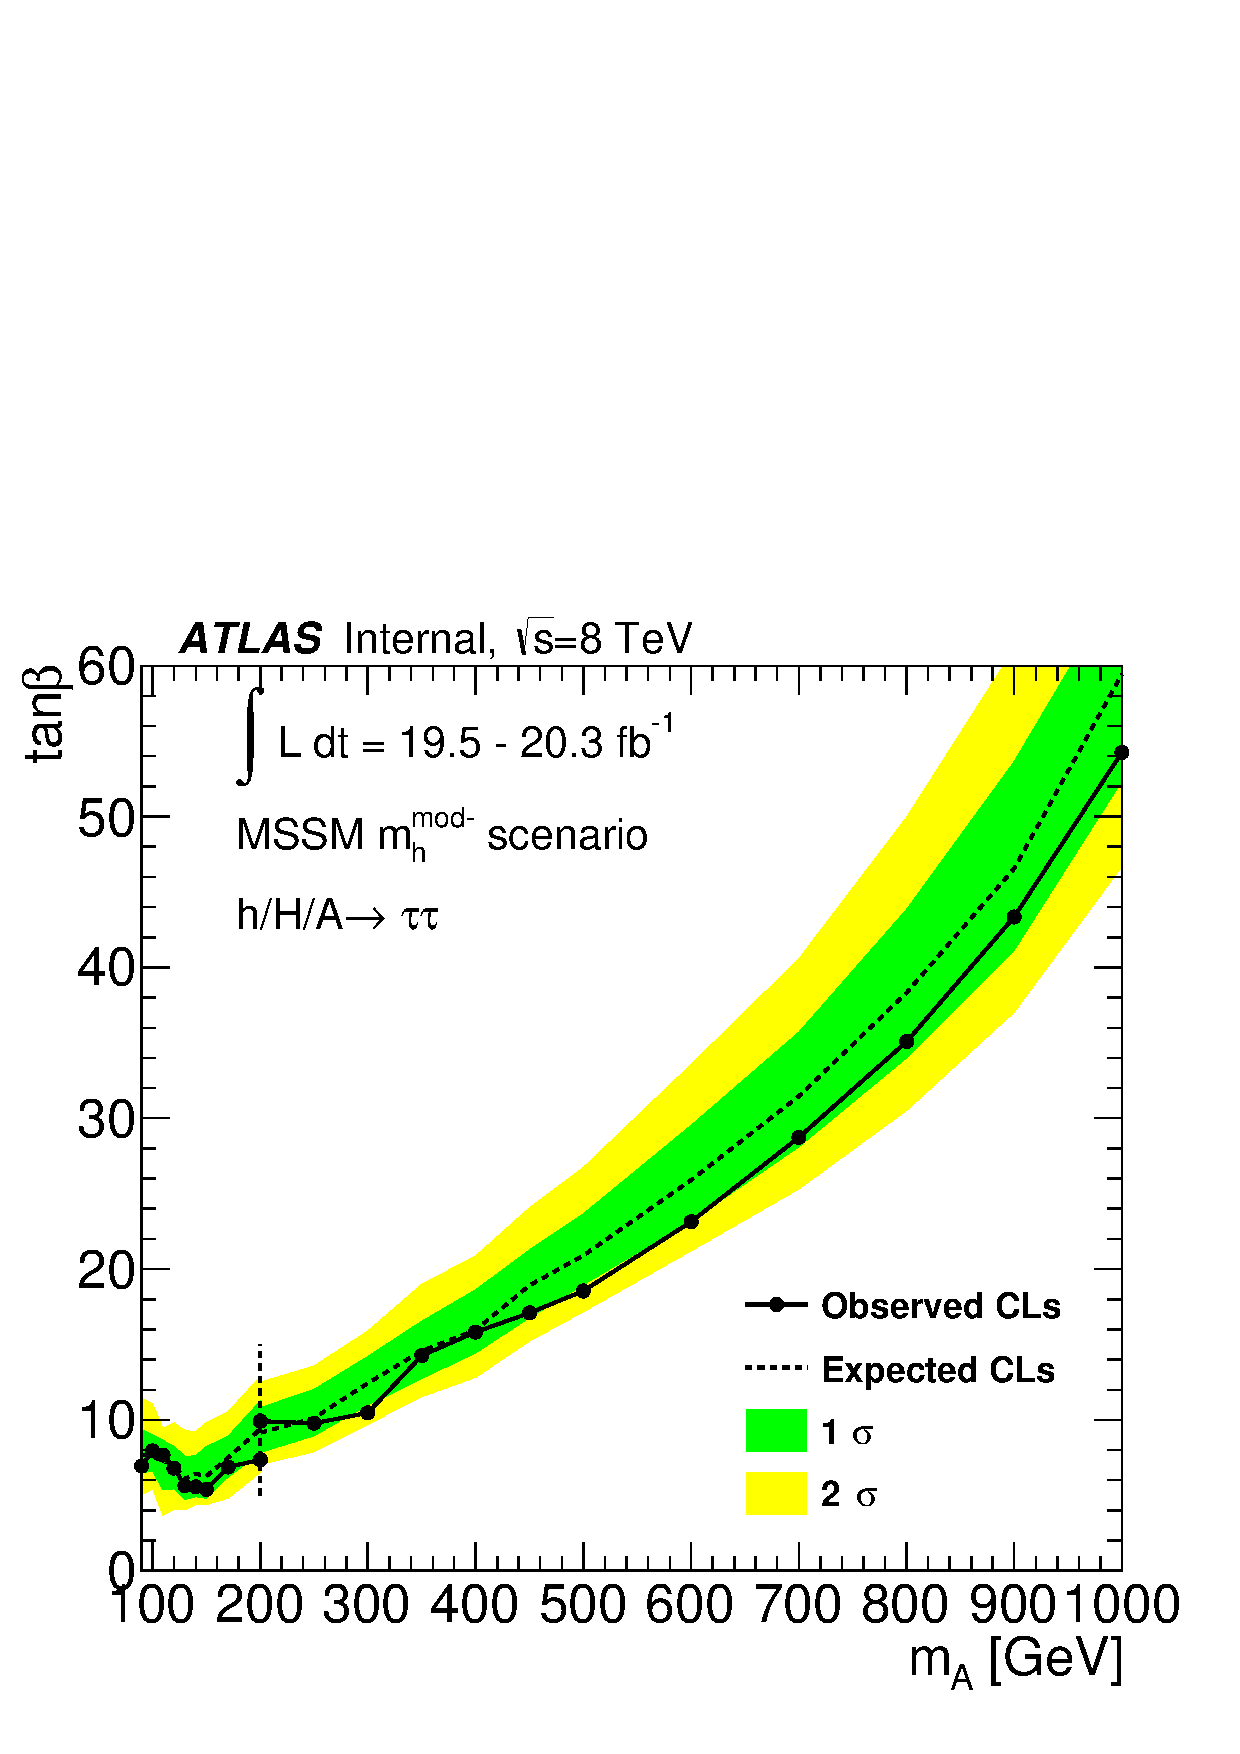
\includegraphics[width=.45\textwidth]{figure/paper/limit_comb_2d_mhmodm.pdf}
%  }
%  \subfigure[light stau]{
%    \includegraphics[width=.45\textwidth]{figure/paper/limit_comb_2d_lightstau.pdf}
%  }
%  \subfigure[light stau]{
%    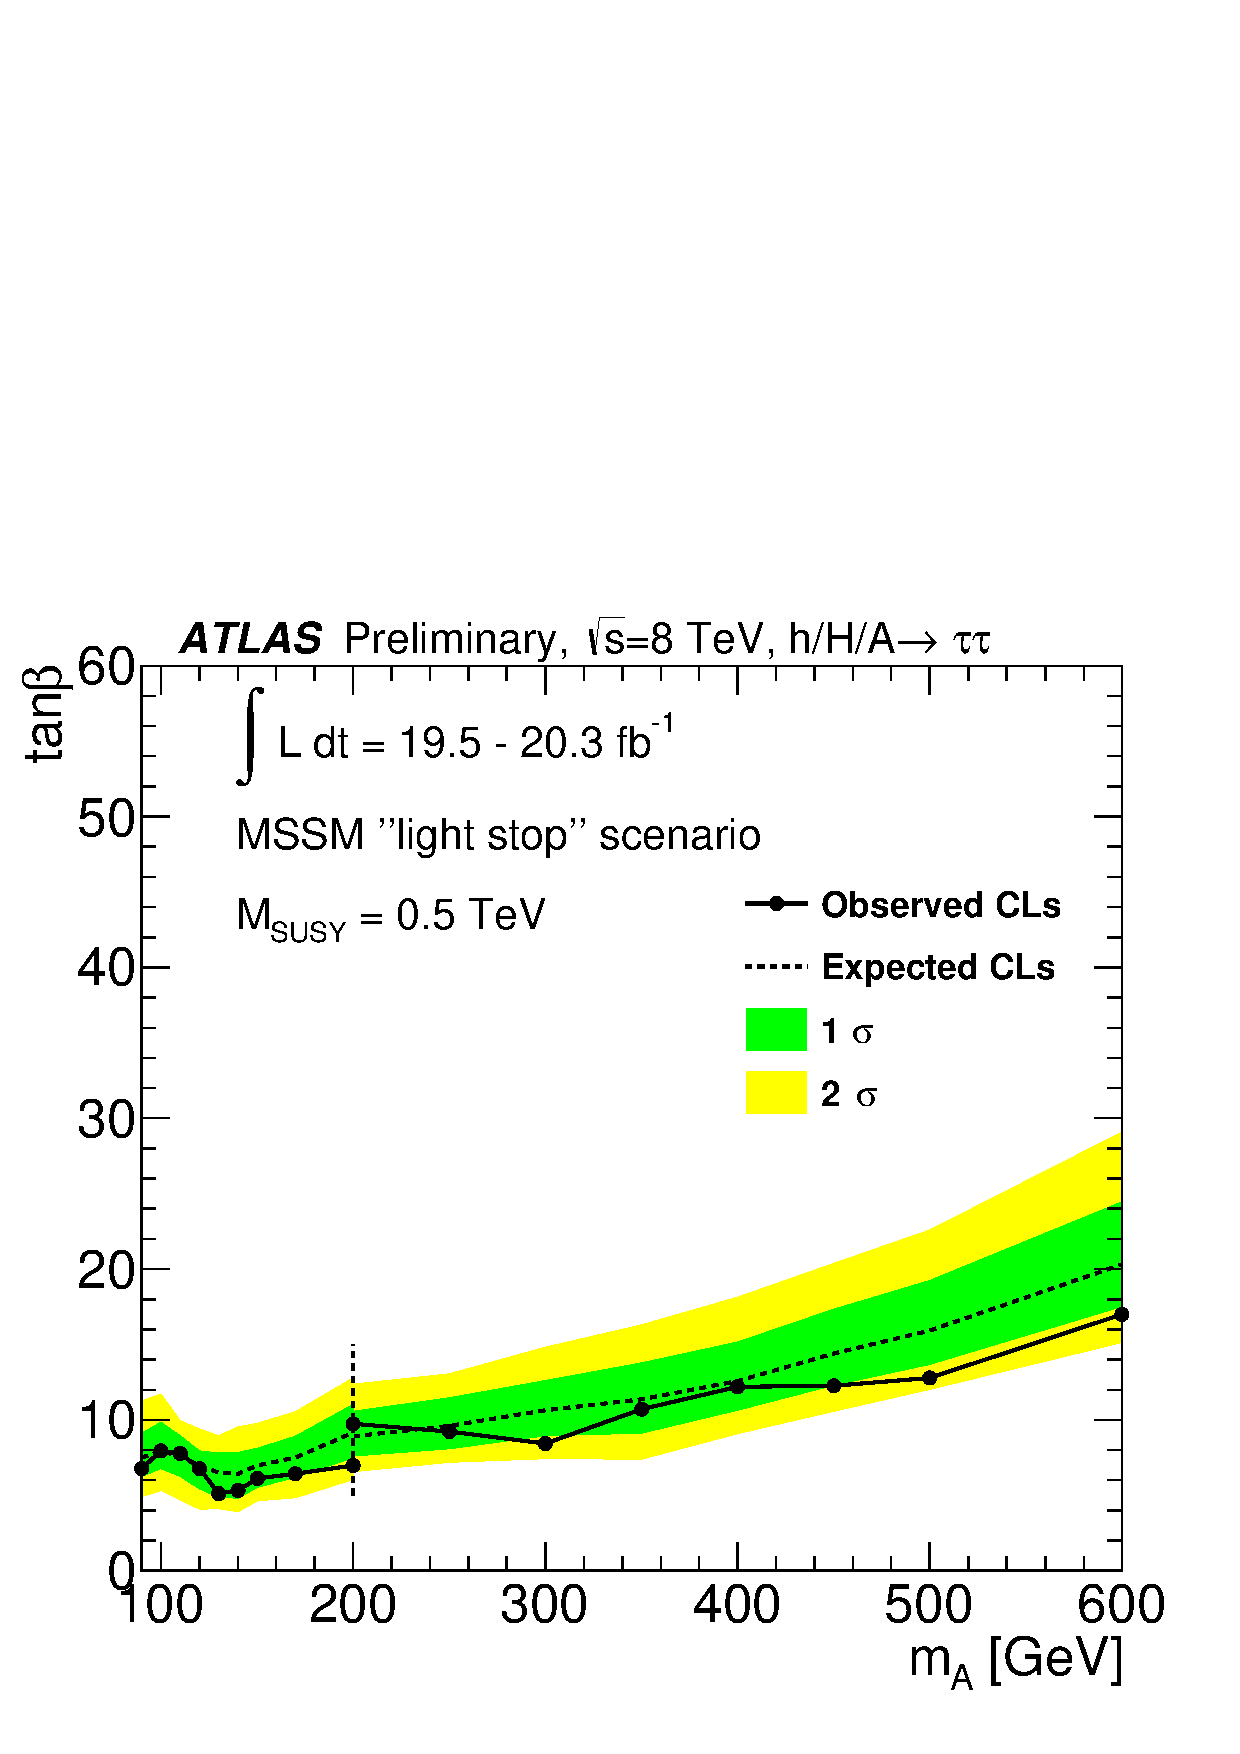
\includegraphics[width=.45\textwidth]{figure/paper/limit_comb_2d_lightstop.pdf}
%  }
%  \subfigure[]{
%    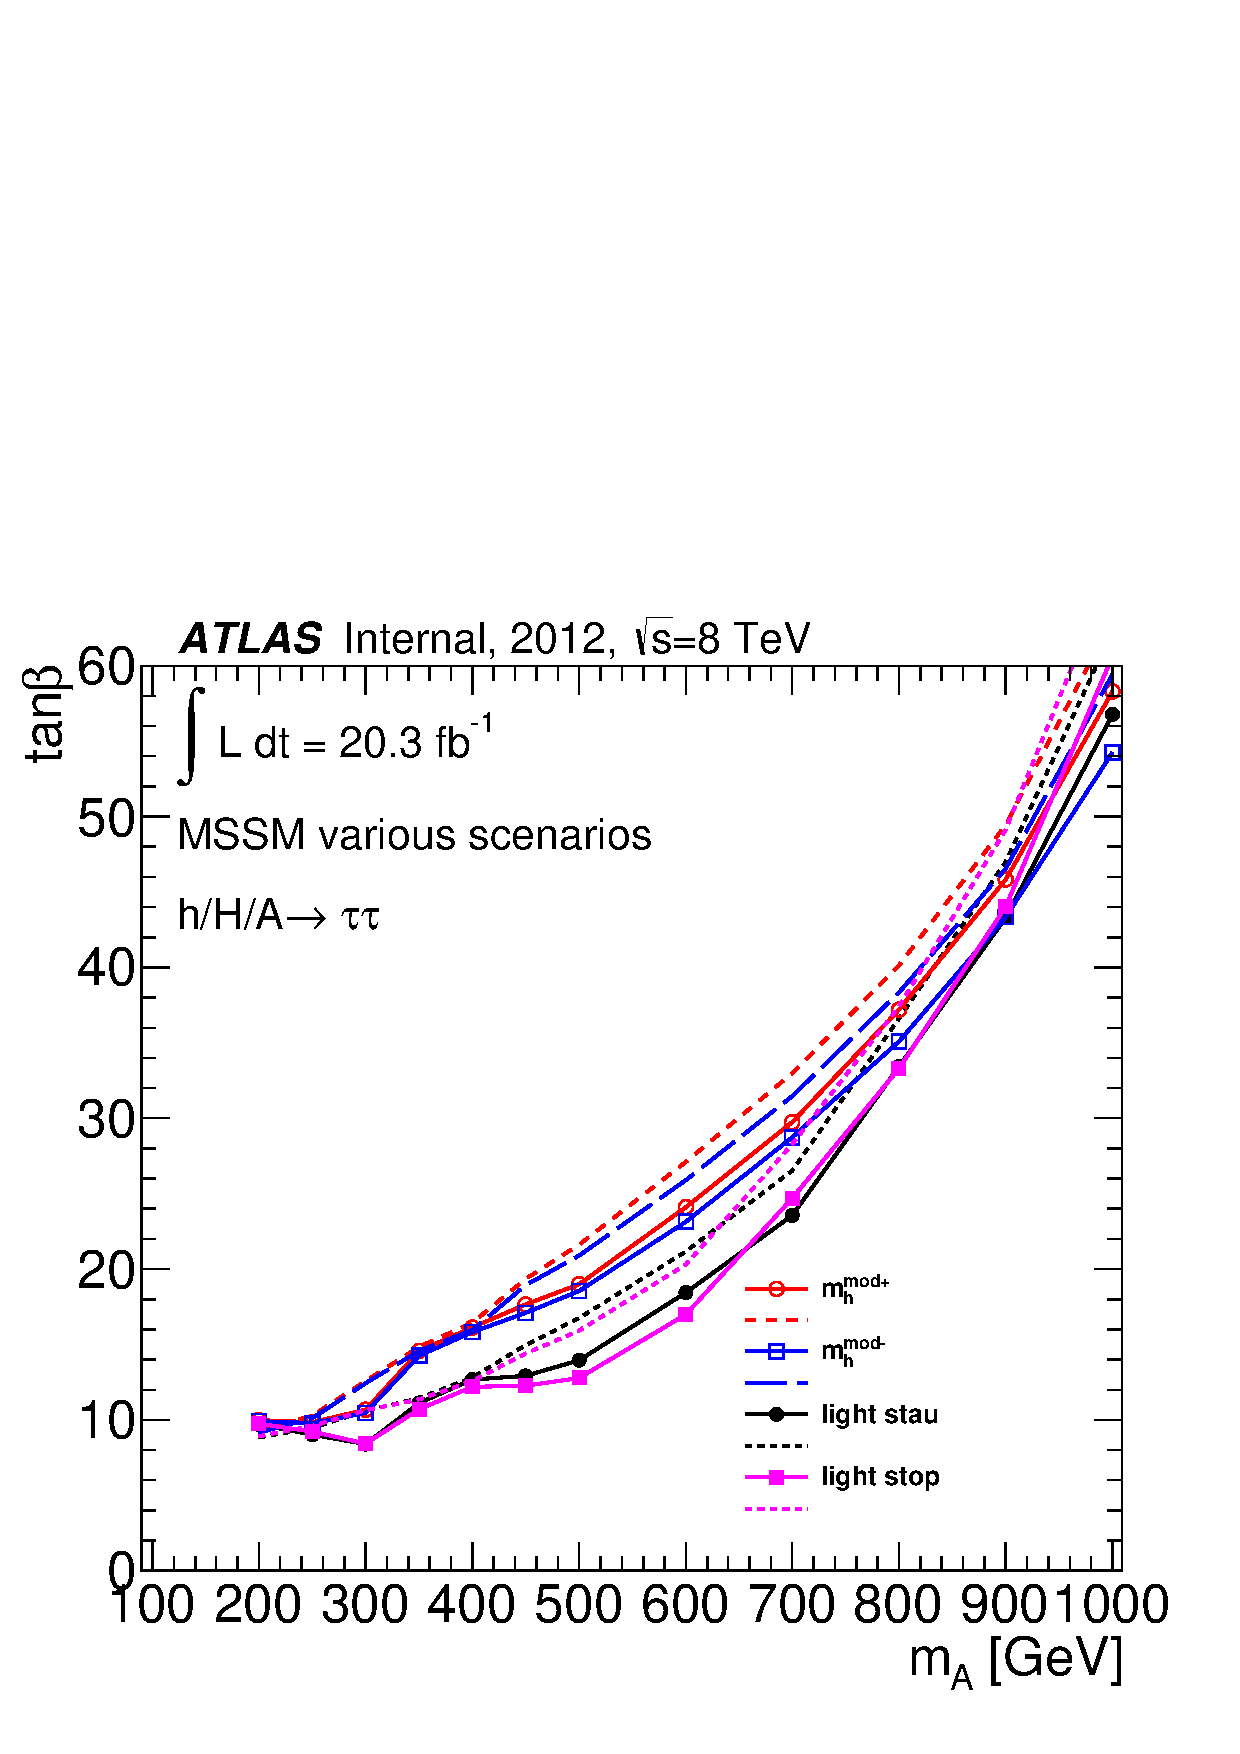
\includegraphics[width=.45\textwidth]{Figures/limits/limit_comb_2d_scenarios.pdf}
%  }
  \caption{
Expected (gray bold line) and observed (black bold line) 95\% CL upper limits
on $\tan\beta$ as a function of $m_A$ for the $m_h^{max}$ scenario~\cite{CMSLimit}.
}
  \label{fig:ex2}
\end{figure}



The constraints on $m_A - \tan\beta$  plane from direct searches for neutral MSSM Higgs bosons searches~\cite{CMSLimit}  are  shown in Figure~\ref{fig:ex2}, the 
$m_h^{max}$ scenario is assumed. 



 




















